% !TEX root = ../termpaper.tex
% first example sections
% @author Thomas Lehmann
%

\section{Grundlagen}
Im folgenden Kapitel wird auf die Grundlagen eingegangen, die in Zusammenhang mit diesem Projekt stehen. Dabei handelt es sich um den bireziproken Teilbandfilter und der Oktav-Filterbank.

\subsection{Bireziproker Teilbandfilter}
Die Grundstruktur des bireziproken Filters sind Wellendigitalfilter. Wellendigitalfilter sind dabei Filter der digitalen Signalverarbeitung, die auch unter nicht linearen Bedingungen eine gute Stabilitätseigenschaft aufweisen \cite[vgl.][S. 68]{gaszi1983}.\par
Bei den bireziproken Filtern, auch selbstreziproke Filter genannt, handelt es sich um eine Unterklasse der Wellendigitalfilter. Bei dem Filterdesign dieser Filter kann entweder die Durchlassdämpfung oder die Sperrdämpfung frei gewählt werden, da der Frequenzbereich bis $\frac{F_s}{4}$ nicht unabhängig von dem Bereich von $\frac{F_s}{4}$ bis $\frac{F_s}{2}$ ist \cite[vgl.][S. 72]{gaszi1983}.\par
Die Anzahl der Adaptoren innerhalb des Filters ist dabei geringer als bei üblichen Wellendigitalfiltern. Bireziproke Filter umfassen $\frac{N - 1}{2}$ Adapter \cite[vgl.][S. 73]{gaszi1983}.\par
Für dieses Projekt wird der bireziproke Filter aus \cite{gaszi1983} verwendet. Hierbei handelt es sich um einen Filter 19. Grades mit Cauer-Parametern. Das Filterdesign und die Berechnung der Cauer-Parameter ist in \cite[][S. 74]{gaszi1983} zu finden.\par
Die Grundstruktur des Filters setzt sich wie in Abbildung \ref{fig:bireziprok_Struktur} aus neun Adaptoren zusammen. Da es bei der Simulation zu keinem Überlauf der Variablen kommen kann und in diesem Zusammenhang die Größe der berechneten Cauer-Parameter keine Auswirkung hierauf haben, wird die Filterstruktur vereinfacht, indem neun gleiche Adaptore verwendet werden. Hierfür wird der Adaptor für einen $\gamma$-Bereich von $0\leq\gamma\leq0,5$ verwendet, da hier die Beziehung von $\alpha=\gamma$ gilt (siehe Abbildung \ref{fig:Adaptor}).
\begin{figure}[h!]
	\centering	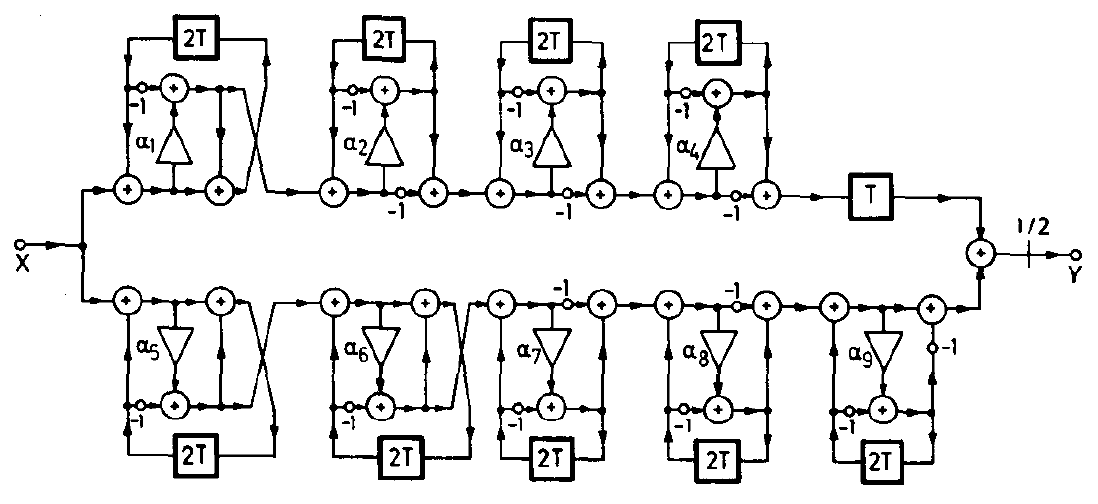
\includegraphics[width=15cm]{img/BireziprokerFilter.png}
	\caption{Grundstruktur des bireziproken Wellendigitalfilters \cite[][S. 85]{gaszi1983}}
	\label{fig:bireziprok_Struktur}
\end{figure}
\begin{figure}[h!]
	\centering	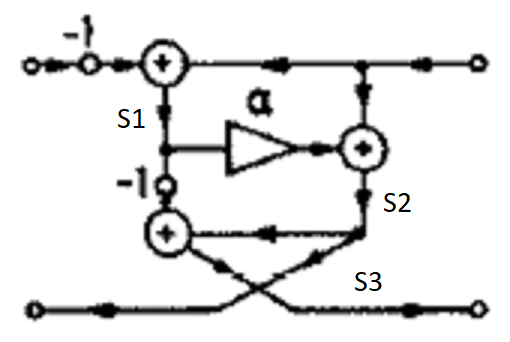
\includegraphics[width=10cm]{img/Adapter.png}
	\caption{Verwendeter Adaptor für den bireziproken Wellendigitalfilter \cite[][S. 77]{gaszi1983}}
	\label{fig:Adaptor}
\end{figure}

\subsection{Oktav-Filterbank}
Bei der Oktav-Filterbank handelt es sich um einen Filter, welcher aus mehreren Brücken-Wellendigitalfiltern besteht. Herbei besitzt jedes Teilbandfilter einen Tief- und Hochpassausgang. Somit ergibt sich, dass je Teilbandfilter das Frequenzband halbiert wird \cite[vgl.][S. 90]{kunold1989}.\par
Um bei jeder Teilbandfilterstufe das Signal jeweils in einen höherfrequenten und niederfrequenten Teil zu trennen, ist eine Filtertransformation nötig. Dies geschieht mit den folgenden Beziehungen:
\begin{equation}
\psi = \frac{z - 1}{z + 1}
\end{equation}
\begin{equation}
\psi' = \frac{2 \psi}{1 + \psi^2} = \frac{2 \left(\frac{z - 1}{z + 1}\right)}{1 + \left(\frac{z - 1}{z + 1}\right)^2} = \frac{z^2 - 1}{z^2 - 1}
\end{equation}
\begin{equation}
z' = z^2
\end{equation}
\begin{equation}
z^{'-1} = z^{-2}
\end{equation}
Somit folgt, dass mit jeder Teilbandfilterstufe die jeweiligen Delays des Filters verdoppelt werden.\par
Da bei jedem Teilfilterdurchlauf ein zusätzlich Delay erzeugt wird, besitzen die neun Teilbänder unterschiedliche Signallaufzeiten. Dies muss durch zusätzliche Delayglieder in den Teilbändern kompensiert werden, damit am Aus- und Eingang der Oktav-Filterbank ein identisches Signal anliegt.\par
Für dieses Projekt wird eine Oktav-Filterbank mit neun Teilbändern nach \cite[][]{kunold1989} verwendet (siehe Abbildung \ref{fig:OktavFilterbank}). Des Weiteren werden die linearphasigen Teilbandfilter gegen bireziproke Teilbandfilter ausgetauscht.
\begin{figure}[h!]
	\centering	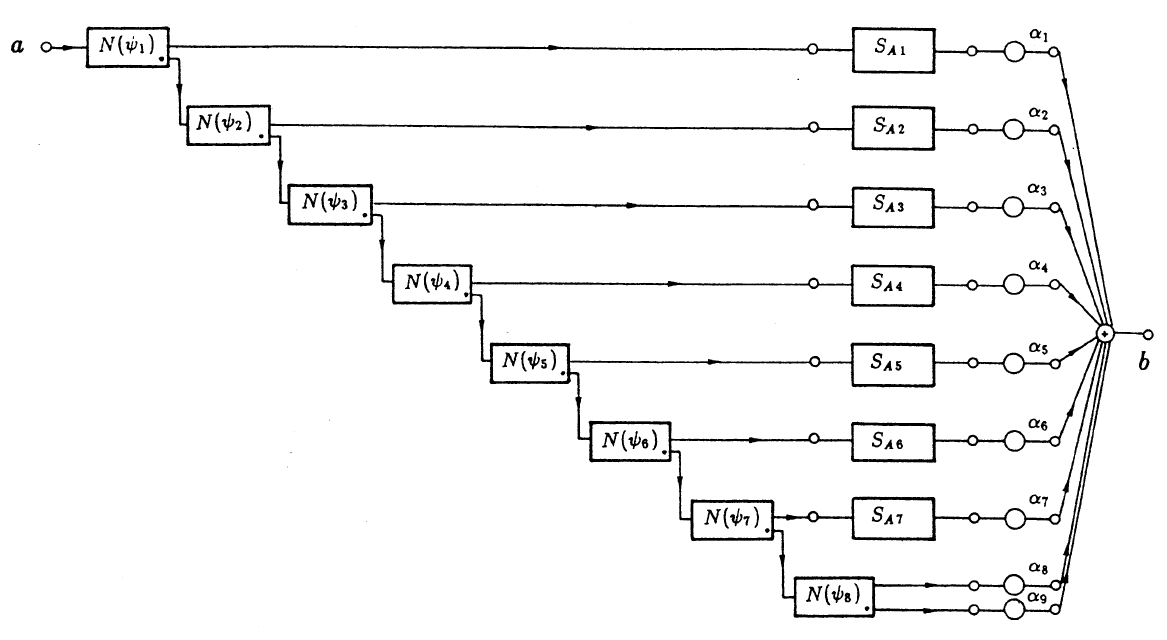
\includegraphics[width=15cm]{img/OktavFilter.png}
	\caption{Oktav-Filterbank mit neun Teilbändern \cite[][S. 95]{kunold1989}}
	\label{fig:OktavFilterbank}
\end{figure}
%%% Local Variables:
%%% mode: latex
%%% TeX-master: "../termpaper"
%%% End:
